\documentclass{article}
\usepackage[utf8]{inputenc}
\usepackage{amsthm}
\usepackage{natbib}
\usepackage{graphicx}
\usepackage{tikz}
\usetikzlibrary{arrows}

% COMMANDS
\newcommand{\basis}{\newline \noindent {\bf Basis:} }
\newcommand{\ih}{\newline \noindent {\bf Induction hypothesis:}  Assume }
\newcommand{\is}{\newline \noindent {\bf Induction:} }


\begin{document}
Alice and Bob are discussing a graph that has 
$17$ vertices and $129$ edges. 
Bob argues that the graph is Hamiltonian, 
while Alice says that he's wrong. 
Without knowing anything more about the graph, 
must one of them be right? If so, who and why, 
and if not, why not?\\

\begin{center}
    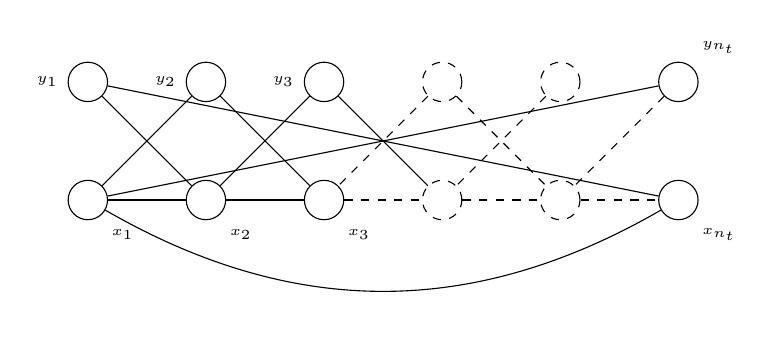
\begin{tikzpicture}[auto,node distance=1.5cm,
        minimum size=.5cm,
        main node/.style={circle,draw}]
    
        \node[main node] [label={left:\tiny{$y_3$}}] (y3) {};
        \node[main node] [label={left:\tiny{$y_2$}}] (y2) [left of=y3] {};
        \node[main node] [label={left:\tiny{$y_1$}}] (y1) [left of=y2] {};
        \node[main node] [dashed] (y4) [right of=y3] {};
        \node[main node] [dashed] (y5) [right of=y4] {};
        \node[main node] [label={above right:\tiny{$y_{n_t}$}}] (yn) [right of=y5] {};
        \node[main node] [label={below right:\tiny{$x_1$}}] (x1) [below of=y1] {};
        \node[main node] [label={below right:\tiny{$x_2$}}] (x2) [right of=x1] {};
        \node[main node] [label={below right:\tiny{$x_3$}}] (x3) [right of=x2] {};
        \node[main node] [dashed] (x4) [right of=x3] {};
        \node[main node] [dashed] (x5) [right of=x4] {};
        \node[main node] [label={below right:\tiny{$x_{n_t}$}}] (xn) [right of=x5] {};
    
        \path[every node/.style={font=\sffamily\small}]
        (x1) edge node {} (x2)
        (x2) edge node {} (x3)
        (x3) edge [dashed] node {} (x4)
        (x4) edge [dashed] node {} (x5)
        (x5) edge [dashed] node {} (xn)
        (xn) edge [bend left] node {} (x1)
        (y1) edge node {} (x2)
        (y1) edge node {} (xn)
        (y2) edge node {} (x1)
        (y2) edge node {} (x3)
        (y3) edge node {} (x2)
        (y3) edge node {} (x4)
        (y4) edge [dashed] node {} (x3)
        (y4) edge [dashed] node {} (x5)
        (y5) edge [dashed] node {} (x4)
        (yn) edge [dashed] node {} (x5)
        (yn) edge node {} (x1)
        ;
    \end{tikzpicture}\\
\end{center}

\bibliographystyle{plain}
\bibliography{references}
\end{document}